%\section{Distribution of IVOA Virtual Observatories Worlwide and its Projects}
\section{IVOA Virtual Observatories}
\label{sec:ivoa}

Astronomy has always been a data-driven science, and therefore,
the digital revolution have completely change the astronomical practice.
In fact, the actual presence of the astronomer on site is every
day less required for performing observations, and data reduction process
is migrating out of the observatories, and international data sharing
and collaboration are becoming common practices in the community.

However, the paradigm change 
does not stop here, because astronomers have to front the main challenge of
21st century science: the data deluge. It is a fact that astronomical data will
strongly increase both in size and in quantity on the next decade due to various
reasons, including the building of large projects like ALMA and E-ELT, 
the improvement and deployment of new instruments, and the execution of 
large astronomical surveys like the LSST project.
The effort needed to process all this data will be enormous both
scientifically and in terms of computational capacity. 
For instance, simple search and access procedures could become highly expensive
when too many files are available in the database.

Consequently, is desirable to distribute the scientific and the computational 
load in several centers, each one specialized on certain data and instruments
to avoid redundancy of observations and work. However, this distributed work
should be organized to be able to interoperate between centers.
In this context, organizing the inherent diversity of several countries working together, 
with different goals, working-style and budgets is the central objective of
the IVOA.


\scriptsize
\begin{table}[h]
\centering
%\begin{tabular}{|p{7cm}|p{7cm}|}
\begin{tabular}{|l|l|l|}
	\hline
	\textbf{Project} & \textbf{Since} & %\textbf{Organization} & % \textbf{Institutions Acronyms} & 
\textbf{URL} \\
	\hline
	Aus-VO (Australia) & 2002 & %Partnership of 10 Universities/Institutes  & 
		\url{http://aus-vo.org.au/} \\
	\hline
   CVO (Canada) & 2002 & %Governmental Initiative + 1 partner & % CADC, NRC, CSA &
   	\url{http://www.cadc-ccda.hia-iha.nrc-cnrc.gc.ca} \\
%	EURO-VO (Europe) & 
%& & \url{http://www.euro-vo.org/} \\
	\hline
	GAVO (German) & 2002 & % Partnership of 5 Universities/Institutes &   
		\url{http://www.g-vo.org/} \\
	\hline
	VO-France (France) & 2002 & % & 
		\url{http://www.france-vo.org/} \\
	\hline
	RVO (Russia) & 2002 & % &  
		\url{http://www.inasan.rssi.ru/eng/rvo/} \\
	\hline
	US-VAO (United States) & 2002 & %  &
		 \url{http://www.usvao.org/} \\
	\hline
	VOI (India) & 2002 & %  & 
		\url{http://vo.iucaa.ernet.in/~voi/} \\
	\hline
	AstroGrid (UK) & 2002 & %Consortium of 7 University/Institutes & %CU,EU,LU,UM,RAL,UCL,UB & 
		\url{http://www.astrogrid.org/} \\
	\hline
   China-VO (China) & 2003 & % Partnership of 4 Universities/Institutes  & 
   \url{http://www.china-vo.org/} \\
	\hline
	JVO (Japan) & 2003 &% &  
		\url{http://jvo.nao.ac.jp/}\\
	\hline
	VObs.it (Italy) & 2003 & % & 
		\url{http://vobs.astro.it/} \\
	\hline
	HVO (Hungary) & 2003 & %&
 		\url{http://hvo.elte.hu/en/} \\
	\hline
	SVO (Spain) & 2005 & % &  
		\url{http://svo.cab.inta-csic.es/} \\
	\hline
	ARVO (Armenia) & 2006 & %Observatory Initiative + 1 partner & % BAO, ANAS & 
		\url{http://www.aras.am/Arvo/arvo.htm} \\
	\hline
	BRAVO (Brazil) & 2009 & %Governmental Initiative + 4 partners &  %INCT-A,MCT,USP,UFSC,LNA & 
		\url{http://www.lna.br/bravo/} \\
	\hline
	UkrVO (Ukraine) & 2011 & % &  
		\url{http://www.ukr-vo.org/} \\
	\hline
	NOVA (Argentina) & 2011 & %Governmental Initiative + 9 partners  & % CONICET,CASLEO,IALP,IAFE,OAC,IAR,ICATE,UNPL,IATE & 
		\url{http://nova.conicet.gov.ar/} \\
	\hline
	SA$^3$ (South Africa) & 2013 & %  & 
		\url{http://www.sa3.ac.za/} \\
	\hline
    ChiVO (Chile) & 2013 & %Partnership of 7 Universities/Institutes & %UTFSM,UChile,PUC,UdeC,USACH,REUNA,ALMA & 
		\url{http://www.chivo.cl/} \\
	\hline
\end{tabular}
\caption{IVOA's partners.}
\label{table:partners}
\end{table}
\normalsize

\subsection{The IVOA}

Since June 2002, different virtual observatory projects have come to integrate the
International Virtual Observatory Alliance (IVOA) under the \textbf{Guidelines
for
Participation\footnote{\url{http://www.ivoa.net/documents/latest/IVOAParticipation.html}}}. 
These projects are funded through national and international programs, both governmental and 
private, in collaboration with various centers of scientific studies, universities and
others institutions. The members of the Virtual Observatory share
knowledge between them and the community in a standardized manner. They
themselves are who develop these standards for data exchange and
interoperability.
Table \ref{table:partners} shows the partners of IVOA up to
November 2014 that represents a nation. Also, two international organizations
are part of the VO, including the European Space Agency VO
(ESA-VO\footnote{http://www.sciops.esa.int/index.php?project=SAT\&page=ESAVOIntro})
and the EURO-VO~\footnote{http://www.euro-vo.org/}, which is a federation of several VOs in Europe.

\subsection{IVOA Architecture}

A Virtual Observatory (VO) is a framework that helps to solve several
problems faced by the world wide astronomical community.
One of this problems is related to have access to generated data by
different instruments. Therefore, an architecture
\footnote{\texttt{http://www.ivoa.net/documents/Notes/IVOAArchitecture/}} was designed by the IVOA, which is composed by
standards and protocols, that allow the transparent
and unified access to astronomical data servers. The IVOA Architecture
defines 3 layers:
\begin{itemize}
        \item the \textbf{Resource Layer} consists in a server
collection with data from different instruments,
        \item the \textbf{User Layer} where astronomers and researchers can
search for data through different mechanisms,
        \item and the \textbf{Middle Layer} which allows the connection
between the previous two layer, hiding all the complexity for the
users. Thus, they can find data through the \emph{Registry}, or get the data
through \emph{Data Access} protocols.
\end{itemize}

\begin{figure}%[h]
\begin{center}
	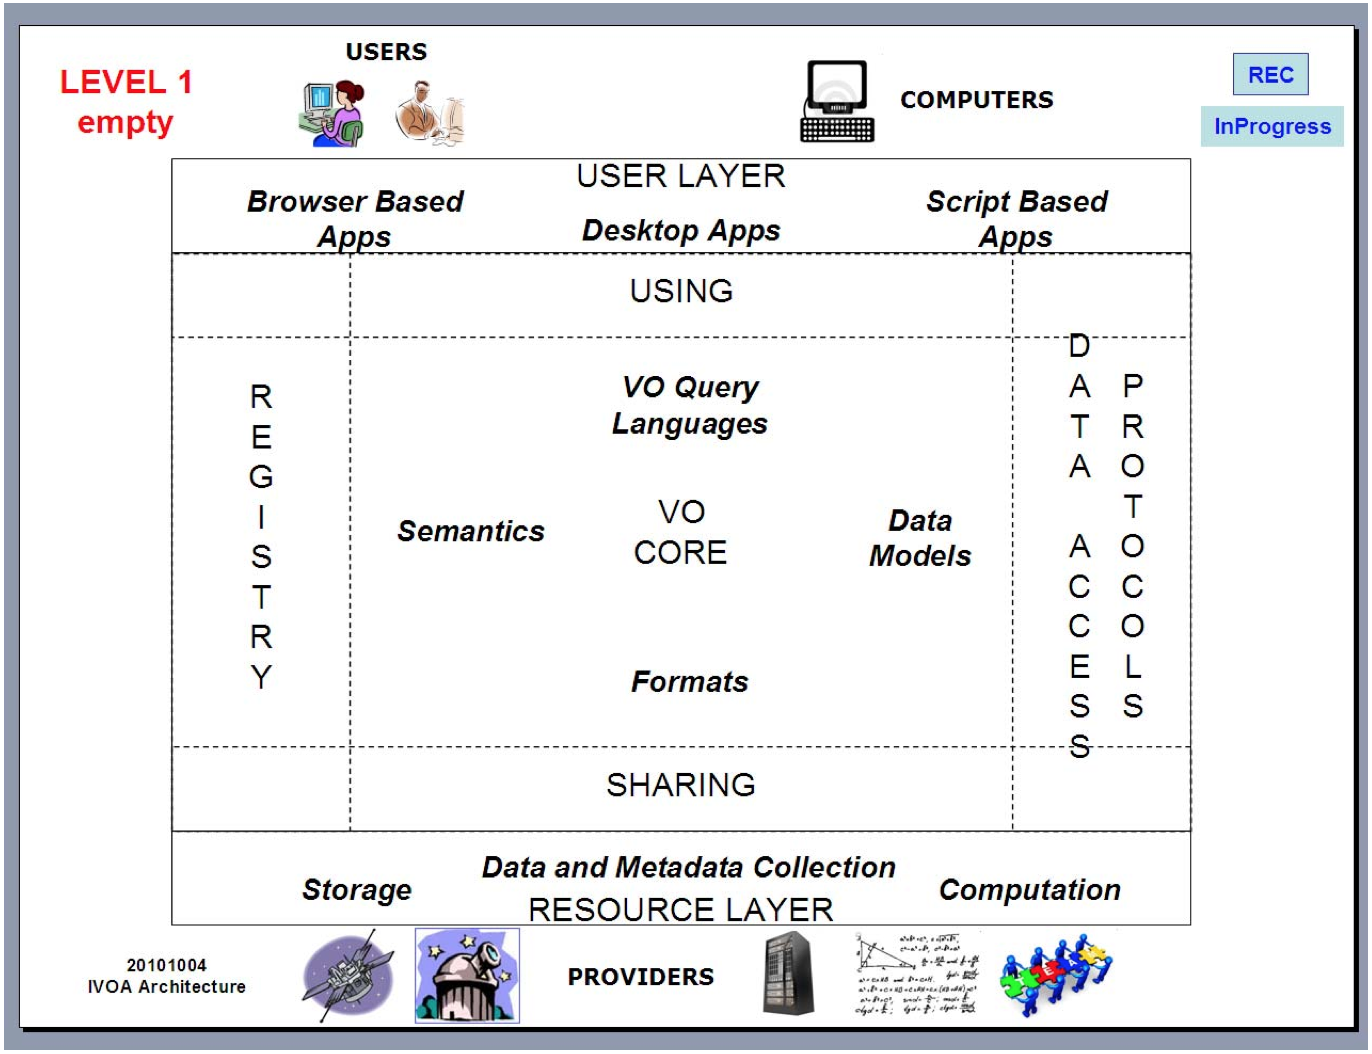
\includegraphics[width=0.9\linewidth]{img/ivoa_arch.png}
	\caption{IVOA Architecture.}
\end{center}
\label{figure:ivoarch}
\end{figure}

\subsection{Working groups}

For the creation and update of standards and protocols, IVOA is organized
by working groups. The description of each standard can be
found in IVOA website\footnote{http://www.ivoa.net/members/}. 
Currently, IVOA is organized in the following \textbf{Working Groups}:
\begin{itemize}
\item \textbf{Applications}:it is concerned primarily with the software
	tools that astronomers use to access VO data an services.
\item \textbf{Data Access Layer}: define and formulate VO standards for
	remote access, oriented to publishers and clients functionalities.
\item \textbf{Data Modeling}: provide a framework for the description
	of metadata attached to observed or simulated data.
\item \textbf{Grid and Webservices}: define the use of grid technologies
	and web services within the VO context.
\item \textbf{Resource Registry}: allow an astronomer to be
	able to locate, get details, and use, any resource located 
	anywhere in the VO.
\item \textbf{Semantics}: explore the word  and sentences
	meaning or interpretation, or another language forms in the
	astronomical context.
\item \textbf{VO Event}: define the content and meaning of a
	standard information packet for representing, transmitting, 
	publishing and archiving information about a transient celestial event.
\item \textbf{VOTable}: maintenance of an XML format, defined
	for the exchange of tabular data in the context of the VO.
\end{itemize}


\subsection{Popular Standard and Services}
\label{sec:popservices}

The working groups described above, have defined several standards
and recommendations that each VO node should implement. A standard usually 
define a basic set of elements to be implemented in order
to be IVOA compliant, but it also define recommendations of optional
elements and protocols. A clear distinction can be made between those
standards that define service protocols, and those that define data models,
semantic descriptions or other internal implementation details.

Currently, the most popular \emph{services} are those defined for
the \textbf{Data Access Layer} (DAL) (right side of Figure~\ref{figure:ivoarch}), 
probably because recovering data is the first thing that a VO node must offer.
We highlight here the four most used ones:
\begin{itemize}
\item \textbf{SCS}: Simple Cone Search, a query that describes a sky position and a
angular distance, defining a cone on the sky where to search for resources.
\item \textbf{SIA}: Simple Image Access, a query that defines a rectangular region on
the sky where to find images.
\item \textbf{SSA}: Simple Spectral Access, an interfaces to remotely discover
and access one-dimensional spectra. 
\item \textbf{TAP}: Table Access Protocol, a service protocol for accessing
general table data. The access is provided for both database and table metadata
as well as for actual table data.
\end{itemize}

On the other hand, identifying the most used ``non-service'' standards is much
more subjective, because specific implementations are much complex to verify
than services, and no all the VO nodes accurately report their IVOA compliance. 
Regardless this, we highlight here four ``non-service'' standard that are usually important
to consider:
\begin{itemize}
\item \textbf{ADQL}: Astronomical Data Query Language, a query language strongly
based on SQL92 that include astronomy specific operations. 
\item \textbf{ObsCoreDM}: Observation Core Data Model, a data structure
containing the basic information used by standard query services such as SCS.
\item \textbf{VOTable}: Virtual Observatory Table, a XML standard for the
interchange of astronomical data represented as a set of tables, loosely based 
in the FITS table standard.
\item \textbf{VOSpace}: Virtual Observatory Space, the IVOA interface to
distributed storage that host persistent and interchangeable data.
\end{itemize}

At last, we want to highlight the important effort made by IVOA in semantics:
it is not enough to have the same data structures and protocols of
communications, the contents of data and metadata should mean the same 
independent of the specific VO in order to have true interoperability.
The semantics working group has developed a standard for Unified Content
Descriptors (UCD), a maintenance protocol of these descriptors, a 
standard vocabulary for the VO, and a standard syntax and semantics for 
units. The importance of developing VO tools with standard semantics goes
beyond machine interoperability, it helps with human interoperability.
A VO-compliant tool should not only get along with VO-services, but also
provide an unified and understandable namespace and context to human users
(i.e. astronomers), allowing more efficient searching, processing and 
visualization.

\subsection{Summary of VO Toolkits}

\begin{table*}[h!t]
   \centering
   \begin{tabular}{|l|l|l|l|l|l|}
   \hline
   \textbf{Toolkit} & \textbf{VO} & \textbf{DAL Services} & \textbf{Language} &
\textbf{Download} & \textbf{Support} \\
   \hline
   \hline
DALToolKit & ESA-VO & SCS/SIA & Java & Available & No\\
   \hline
SVOCat & SVO & SCS            & Unknown & On demand & On demand \\
   \hline
MySpec-MyImg & SVO & SIA/SSA  & Unknown & On demand & On demand \\
   \hline
SAADA & VO-France & SCS/SIA/SSA/TAP & Java & Available & Yes \\
   \hline
DALServer & US-VAO & SCS/SIA/SSA/SLA & Java & Available & No \\
   \hline
VO-Dance & VObs.it & SCS/SIA/SSA & Java/Python & Available & Yes \\
   \hline
DaCHS & GAVO & SCS/SIA/SSA/TAP/Reg & Python & Available & Yes \\
   \hline
OpenCADC & CVO & SCS/SIA/SSA/TAP/Reg & Java/Python & Available & Yes\\
   \hline
DSA & AstroGrid & SCS/TAP & Java & On demand & No \\
  \hline
   \end{tabular}
   \caption{Toolkits}
   \label{table:tk}
\end{table*}

Several VOs have developed their own software packages (known as toolkits)
for publishing data under the IVOA architecture and standards.
IVOA maintains a list of these
toolkits\footnote{\url{http://wiki.ivoa.net/twiki/bin/view/IVOA/PublishingInTheVONew}}, 
which is summarized in table~\ref{table:tk}. Some of these toolkits also include
support for the VOSpace service, but they are usually distributed as a different
toolkit that works similarly to the main one.

